\section{Enti di normazione - standard setting organizations}

\subsection{Natura giuridica degli SSO}
Normalmente si parla di \textit{consorzi}, ossia di associazioni in cui più imprenditori, per mezzo di apposito contratto, costituiscono un'organizzazione comune per la disciplina o per lo svolgimento di determinate fasi delle rispettive imprese.

Tali consorzi sono regolamentati da \textit{statuti} che stabiliscono:
\begin{itemize}
    \item Modalità di accesso
    \item Meccanismi di voto
    \item Meccanismi di sanzione
    \item \dots
\end{itemize}

\subsection{Livelli territoriali degli SSO}
Dal punto di vista europeo ci sono tre livelli:
\begin{itemize}
    \item Livello nazionale: quasi tutti i Paesi del mondo sono dotati di SSO a livello nazionale che si occupano di rilasciare standard. In Italia i principali enti di normazione sono:
        \begin{itemize}
            \item \textbf{UNI} - Ente Nazionale Italiano di Unificazione: associazione privata senza scopo di lucro i cui soci sono imprese, liberi professionisti, associazioni, istituti scientifici e scolastici, PA. L'associazione si occupa di elaborare norme sviluppate da organi tecnici ai cui lavori partecipano tutti gli interessati, rappresentare l'Italia nelle attività di standardizzazione, \dots \newline UNI partecipa a livello europeo alle attività dell'ISO e del CEN. 
            UNI si suddivide in sotto-enti e nel mondo dell'informatica, in particolare, esiste l'\textbf{UNINFO}
            \item \textbf{CEI} - Comitato Elettronico Italiano: si occupa del settore della diffusione della cultura tecnica e della sicurezza elettrica. 
        \end{itemize}
    \item Livello europeo:
        \begin{itemize}
            \item \textbf{CEN} - Comitato Europeo di Normazione: equivalente dell'UNI a livello europeo. La sua attività è coordinata con quella di \textbf{ETSI} (analogo all'UNINFO) e \textbf{CENELEC} (analogo al CEI)
            \item \textbf{ECMA}
        \end{itemize}
    \item Livello internazionale: 
        \begin{itemize}
            \item \textbf{ISO}
            \item \textbf{IEC}
            \item \textbf{ITU-T}: sezione dell'ITU che si occupa delle standardizzazioni
        \end{itemize}
\end{itemize}

ISO e IEC collaborano in comitati tecnici congiunti (\textbf{JTC}). I JTC sono a loro volta divisi in sotto-comitati e gruppi di lavoro.\bigskip

L'ITU ha una serie di compiti (l'abbiamo già incontrata relativamente al processo di suddivisione dello spettro delle frequenze) relativi anche alla standardizzazione. 
L'ITU nasce come agenzia delle Nazioni Unite, con sede a Ginevra. Anch'essa ha diversi comitati di lavoro.\bigskip

Oggi le attività di ITU-T, ISO e IEC sono congiunte.
Il rapporto tra tutte le organizzazioni è sintetizzato in figura \ref{organismi standardizzazione}.

\begin{figure}
    \centering
    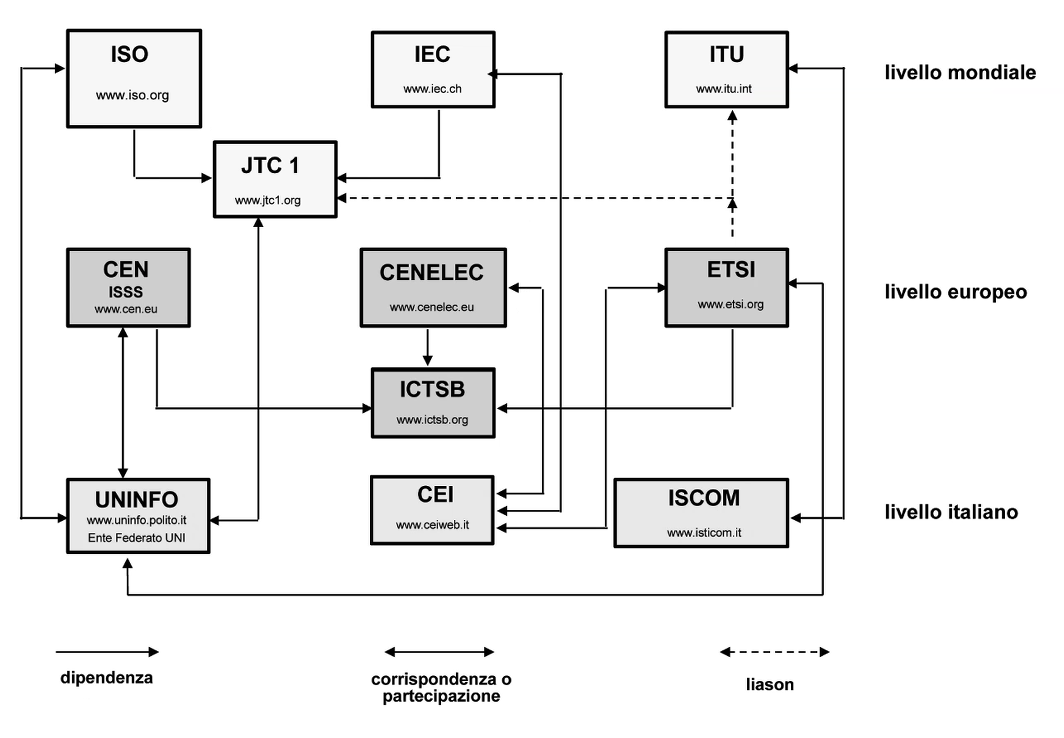
\includegraphics[width=.7\textwidth]{organismi standardizzazione.png}
    \caption{Organismi di standardizzazione}
    \label{organismi standardizzazione}
\end{figure}

